\subsection{Others Tab}

\begin{figure}[H]
   \center
    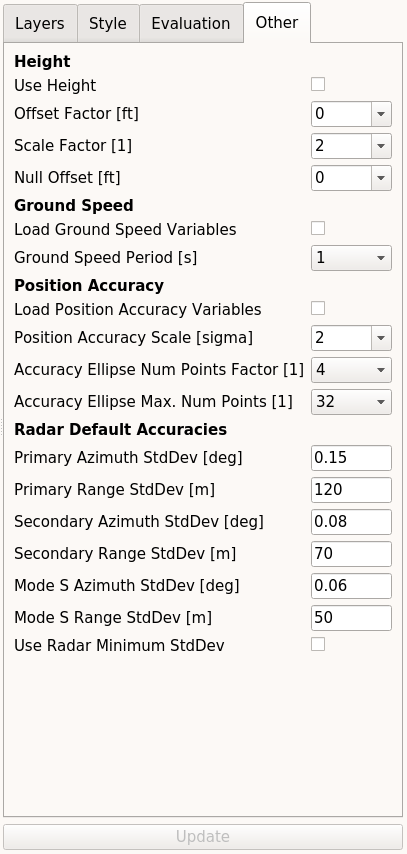
\includegraphics[width=9cm,frame]{figures/geoview_others_tab.png}
  \caption{Geographic View Others tab}
\end{figure}

In the 'Others' tab, several elements exist:

\begin{itemize}
 \item Height: Defines if and how height information is used.
 \item Ground speed: Defines if and how ground speed information is used.
 \item Position Accuracy: Defines if and how position accuracy information is used.
 \item Radar Default Accuracies: Defines Radar default accuracies.
 \item Update button: Triggers a redraw or reload of the geometry, becomes available after a change if needed.
\end{itemize} 

\subsubsection{Height}
\label{sec:others_height}

Per default, a target report's height is not used for display, which is common in current air-traffic displays. However, in certain situations a true 3D display might be of interest to a user, and therefore several options were incorporated:

\begin{itemize}
 \item Use Height: Use the height based on Mode C $h_c$, transformed to meters
 \item Offset Factor: If height information is used, this factor $h_o$ is added to the height
 \item Scale Factor: If height information is used, this factor $h_s$ is used to multiply the height
 \item Null Offset: If height information is used, this factor $h_n$ is used for target reports without height information
\end{itemize}
\ \\

Generally, if no height information is given (no Mode C code), the height is either $0$ or the height offset (if used). That means that those target reports appear to be on the ground. If connection lines are drawn between the ones in the air and those without, a lot of annoying lines are shown. \\

The formula to calculate the height (if existing) is as follows: 

$$ h = h_o + h_s \cdot h_c [m]$$ 

If no height information is given:

$$ h = h_n [m]$$ 

Please note that upon changes to the height usage, a manual redraw has to be performed using the 'Redraw' button.


\begin{figure}[H]
    \hspace*{-2.5cm}
    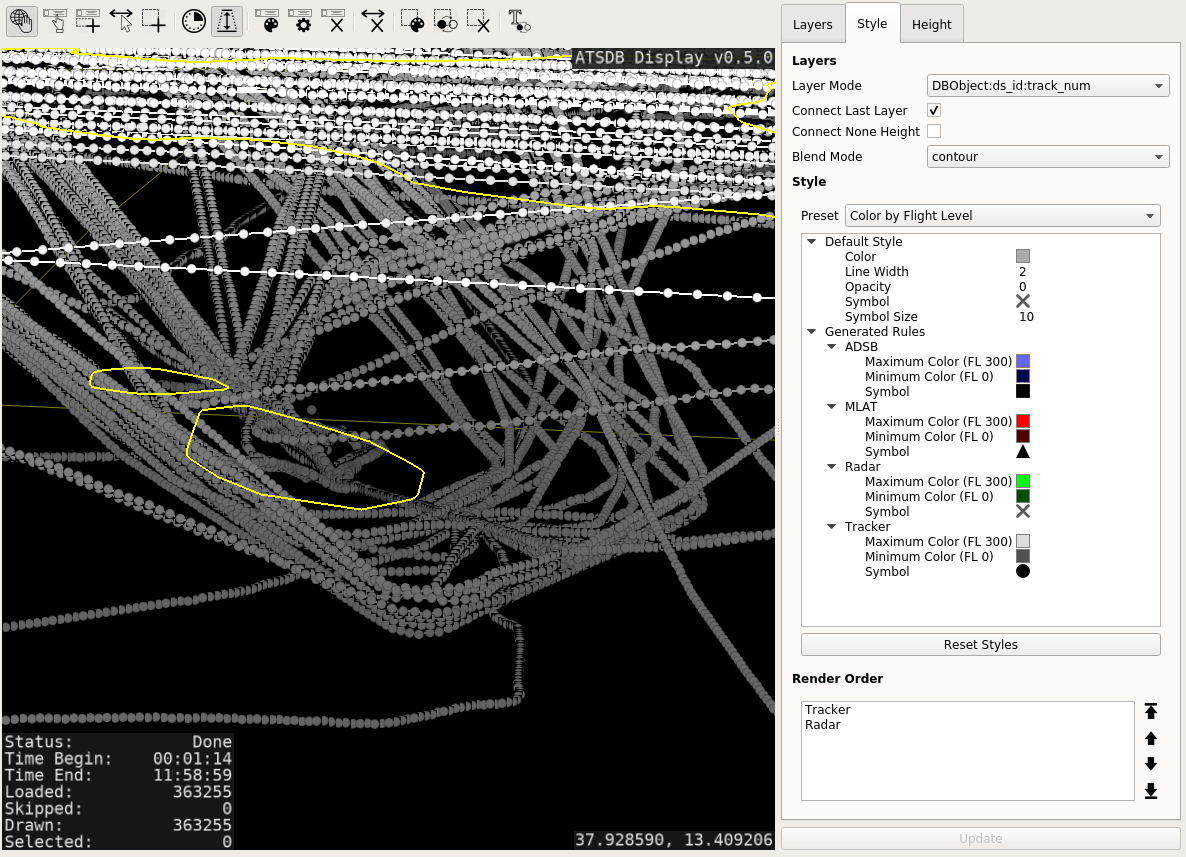
\includegraphics[width=19cm,frame]{figures/geoview_use_height.png}
  \caption{Geographic View use height}
\end{figure} 

\subsubsection{Ground Speed}
\label{sec:others_ground_speed}

\begin{itemize}
 \item Load Ground Speed Variables: Defines if ground speed variables should be loaded from the database. Must be enabled to enable display of ground speed vectors.
 \item Ground Speed Period [s]: Length of ground speed vectors, in seconds.
\end{itemize}
\ \\

If loading is enabled (possible re-load required) the ground speed vectors can be shown using \nameref{sec:geometry_operations}:

\begin{figure}[H]
    \hspace*{-2.5cm}
    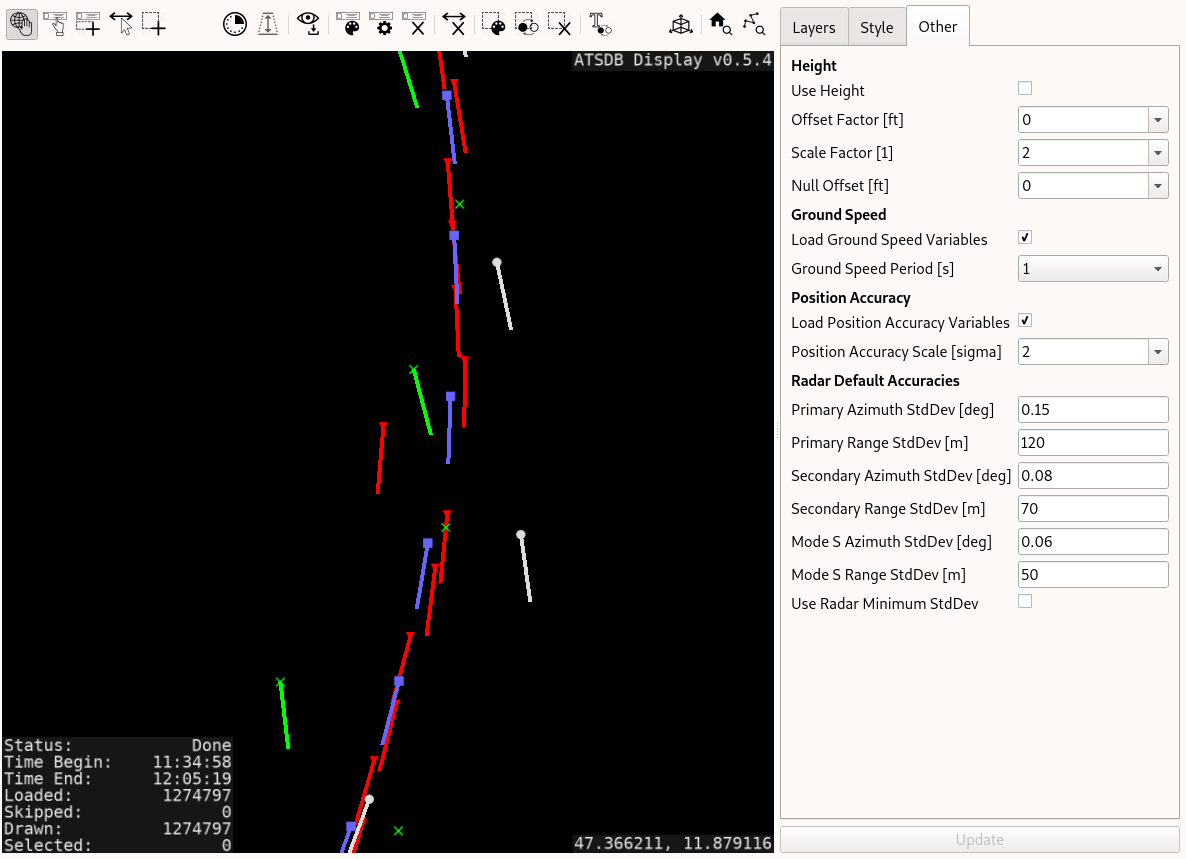
\includegraphics[width=19cm,frame]{figures/geoview_groundspeed_vectors.png}
  \caption{Geographic View groundspeed vectors}
\end{figure} 

\subsubsection{Position Accuracy}
\label{sec:others_position_accuracy}

\begin{itemize}
 \item Load Position Accuracy Variables: Defines if position accuracy variables should be loaded from the database. Must be enabled to enable display of position accuracy ellipses.
 \item Position Accuracy Scale [sigma]: Size of accuracy ellipses, defined in standard deviations:
 \begin{itemize}
    \item 1.0 $\sigma$: 68.268 \%
    \item 1.5 $\sigma$: 86.638 \%
    \item 2.0 $\sigma$: 95.44 \%
    \item 2.5 $\sigma$: 98.75 \%
    \item 3.0 $\sigma$: 99.73 \%
    \item 3.5 $\sigma$: 99.95 \%
    \item 4.0 $\sigma$: 99.9936 \%
    \item 4.5 $\sigma$: 99.999320 \%
    \item 5.0 $\sigma$: 99.99994266 \%
\end{itemize}  
\item Accuracy Ellipse Num Points Factor [1]: Multiplication factor to calculate number of ellipse points based on size
\item Accuracy Ellipse Max. Num Points [1]: Maximum number of ellipse points
\end{itemize}
\ \\

If loading is enabled (possible re-load required) the position accuracy ellipses can be shown using \nameref{sec:geometry_operations}:

\begin{figure}[H]
    \hspace*{-2.5cm}
    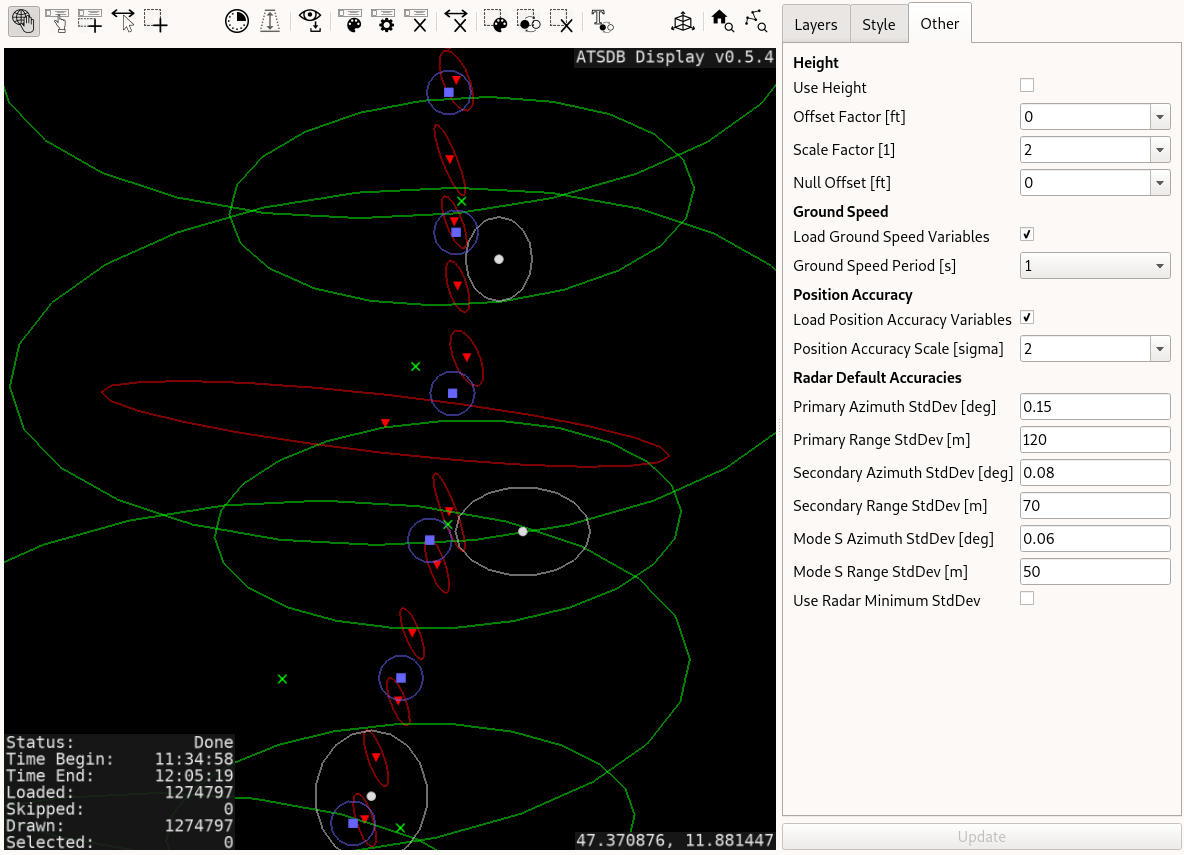
\includegraphics[width=19cm,frame]{figures/geoview_accuracy_ellipses.png}
  \caption{Geographic View position accuracy ellipses}
\end{figure} 

How the position accuracy ellipses are generated is defined in \nameref{sec:algo_position_accuracy_ellipses}.

\subsubsection{Radar Default Accuracies}
\label{sec:others_radar_default_accuracies}

In the following items, the default Radar accuracies can be set:

\begin{itemize}
 \item Primary Azimuth StdDev [deg]: PSR azimuth standard deviation, in degrees
 \item Primary Range StdDev [m]: PSR range standard deviation, in meters
 \item Secondary Azimuth StdDev [deg]: SSR azimuth standard deviation, in degrees
 \item Secondary Range StdDev [m]: SSR range standard deviation, in meters
 \item Mode S Azimuth StdDev [deg]: Mode S Radar azimuth standard deviation, in degrees
 \item Mode S Range StdDev [m]: Mode S Radar range standard deviation, in meters
 \item Use Radar Minimum StdDev: Defines if minimum or maximum standard deviation should be used for combined plots
\end{itemize}
\ \\

These values are only used if the associated data source does not have custom accuracy values set (see \nameref{sec:ui_configure_data_sources}). \\

How the Radar default accuracies are used is defined in \nameref{sec:algo_position_accuracy_ellipses}.

